\subsection{OpenID Connect}

O OpenID Connect (OIDC) é um protocolo para fornecimento de identificação que permite que dados de 
usuários sejam transmitidos de forma segura de um provedor para um cliente, com o consentimento do
usuário. É uma camada sobre o protocolo OAuth 2.0, fazendo uso de todos seus conceitos, 
\emph{tokens} e fluxos, com a adição do fornecimento de atributos do usuário. Esses atributos 
podem ser fornecidos para um sistema por meio de uma API RESTful \texttt{userinfo} ou por meio de 
um \emph{token} de identificação \cite{BIEHL2019}.

O fluxo de código de autorização do OIDC é similar ao fluxo do OAuth 2.0, com a adição do 
\emph{token} de identificação fornecido ao cliente pelo servidor de autorização (chamado de 
provedor OIDC). Este \emph{token} segue o formato JWT e possui declarações sobre a autenticação
de um usuário (Figura \ref{fig:OpenID}). Estas declarações também podem ser acessadas realizando uma 
requisição ao \emph{endpoint} \texttt{userinfo} \cite{OIDCCORE}. 

\begin{figure}[ht]
    \centering
    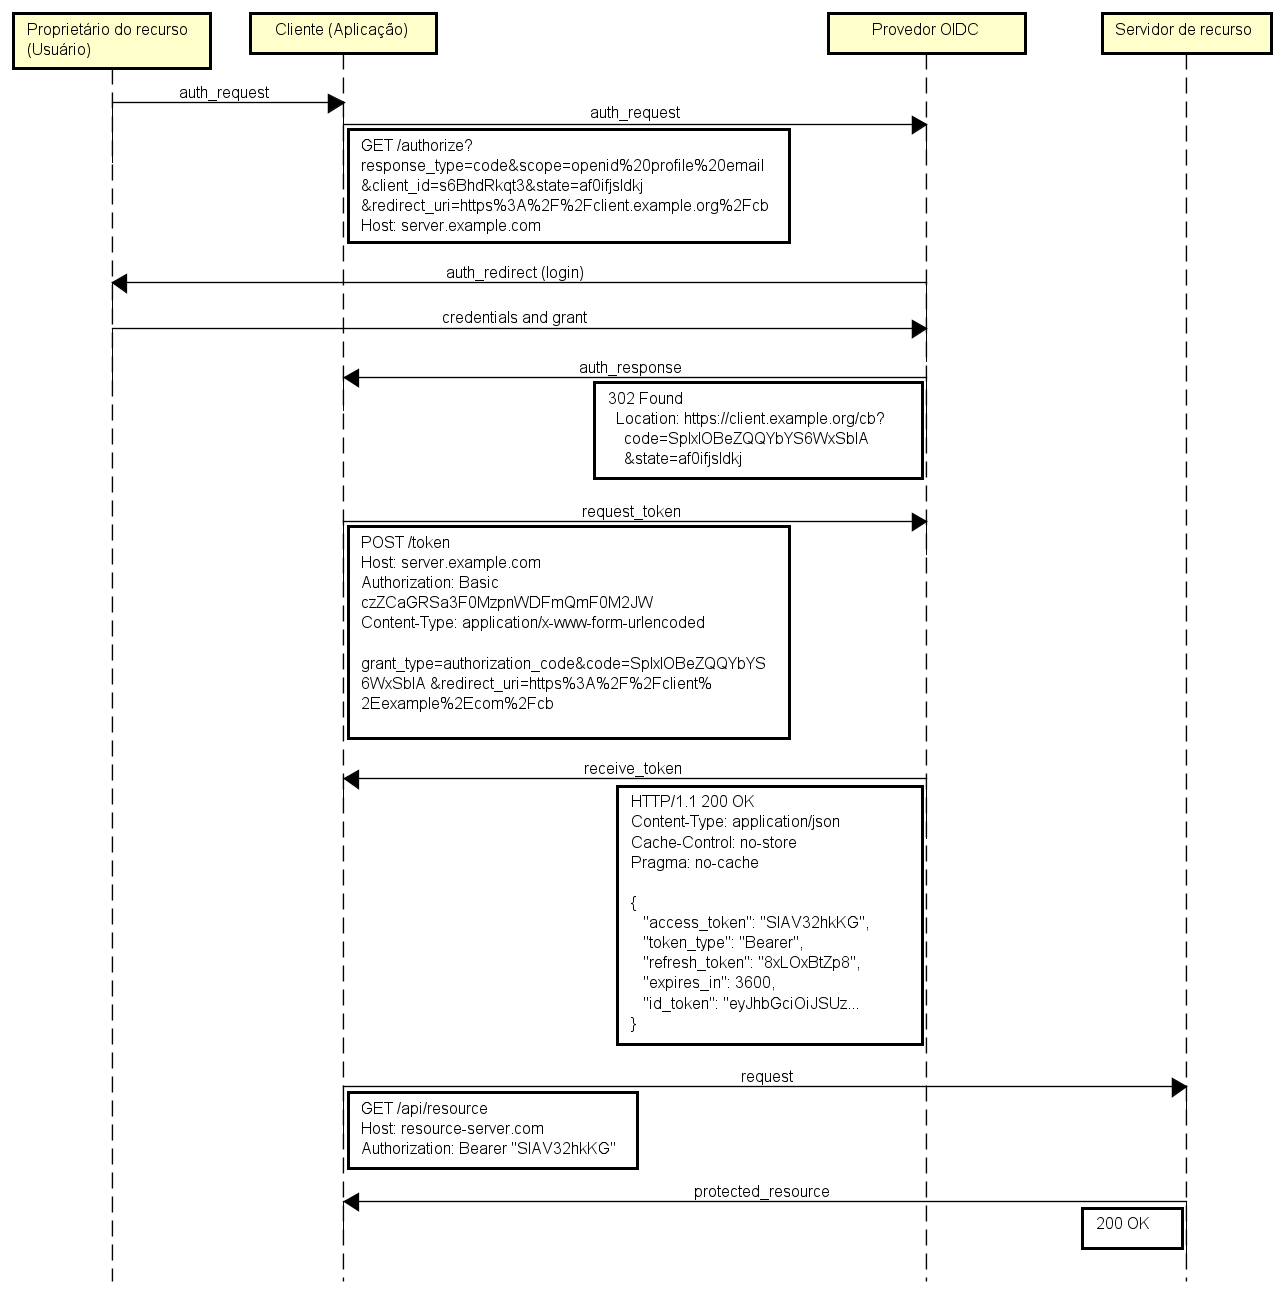
\includegraphics[width=.95\textwidth]{OpenID Connect.png}
    \caption{Exemplo de autenticação utilizando OpenID Connect.}
    \label{fig:OpenID}
\end{figure}